\chapter{Closed-Loop Policy Controller}
\label{ch:controller}

This chapter describes how the fused hallucination-risk probability is used to control the RAG inference loop. Section~\ref{sec:controller_purpose} states the purpose. Section~\ref{sec:controller_inputs} describes inputs and thresholds. Section~\ref{sec:controller_logic} presents the decision logic. Section~\ref{sec:action_semantics} describes the semantic meaning of each action. Section~\ref{sec:trace_ch7} gives an example trace with interpretation, and Section~\ref{sec:ch7_summary} summarizes.

%% -------------------------------------------------
\section{Purpose of the Controller}
\label{sec:controller_purpose}

Chapters~\ref{ch:background}--\ref{ch:probe_training} described how CEV and IAV features are extracted, scored by independent probes, temperature-calibrated, and fused into a hallucination-risk probability. This chapter describes how this probability is used to control the RAG inference loop.

The controller converts hallucination detection into an \emph{inference-time action}. Instead of only assigning a risk score after generation, the controller decides whether the candidate response should be delivered, regenerated, supported by new retrieval, or withheld.

The controller receives three operational inputs:
\begin{itemize}
    \item $p_{\text{fused}}$: the calibrated fused hallucination-risk probability
    \item $q_{\text{ret}}$: the retrieval-quality score (mean similarity of top-$k$ passages)
    \item $r$: the current retry count
\end{itemize}

The controller chooses one of four actions:
\[
    \mathcal{A} = \{\textsc{Accept},\; \textsc{Regenerate},\; \textsc{Re-Retrieve},\; \textsc{Abstain}\}
\]

%% -------------------------------------------------
\section{Controller Inputs and Thresholds}
\label{sec:controller_inputs}

\begin{table}[!htb]
\centering
\caption{Controller threshold symbols.}
\label{tab:threshold_symbols}
\begin{tabular}{@{}lll@{}}
\toprule
\textbf{Symbol} & \textbf{Meaning} & \textbf{Role} \\
\midrule
$\theta_{\text{hallu}}$ & Intervention threshold & Low-risk enough to accept \\
$\theta_{\text{abs}}$   & Abstention threshold & Too risky to continue \\
$\theta_{\text{ret}}$   & Retrieval-quality threshold & Failure caused by weak retrieval \\
\bottomrule
\end{tabular}
\end{table}

In the reported experiments, the retrieval-quality threshold and retry budget are fixed across backbones: $\theta_{\text{ret}} = 0.30$, $\text{MAX\_RETRIES} = 3$.

%% -------------------------------------------------
\section{Controller Decision Logic}
\label{sec:controller_logic}

Let $p_{\text{fused}}$ be the fused hallucination probability, $q_{\text{ret}}$ be the retrieval-quality score, and $r$ be the retry count. The deterministic policy is:

\begin{equation}
\text{Action} = 
\begin{cases}
    \textsc{Abstain}      & \text{if } r \geq \text{MAX\_RETRIES} \\[4pt]
    \textsc{Accept}       & \text{if } p_{\text{fused}} < \theta_{\text{hallu}} \\[4pt]
    \textsc{Abstain}      & \text{if } p_{\text{fused}} \geq \theta_{\text{abs}} \\[4pt]
    \textsc{Re-Retrieve}  & \text{if } \theta_{\text{hallu}} \leq p_{\text{fused}} < \theta_{\text{abs}} \;\wedge\; q_{\text{ret}} < \theta_{\text{ret}} \\[4pt]
    \textsc{Regenerate}   & \text{if } \theta_{\text{hallu}} \leq p_{\text{fused}} < \theta_{\text{abs}} \;\wedge\; q_{\text{ret}} \geq \theta_{\text{ret}}
\end{cases}
\label{eq:controller_rule}
\end{equation}

This rule separates two likely failure sources. If retrieval quality is weak, the system assumes that the model may not have enough reliable evidence and triggers \textbf{RE-RETRIEVE}. If retrieval quality is acceptable but the generated answer remains risky, the system triggers \textbf{REGENERATE} using the same retrieved evidence.

%% -------------------------------------------------
\section{Semantic Meaning of Each Controller Action}
\label{sec:action_semantics}

\begin{table}[!htb]
\centering
\caption{Action semantics.}
\label{tab:action_semantics}
\small
\begin{tabular}{@{}l p{3cm} p{4cm} p{4cm}@{}}
\toprule
\textbf{Action} & \textbf{Trigger} & \textbf{Meaning} & \textbf{System Behavior} \\
\midrule
\textbf{ACCEPT} & $p_{\text{fused}} < \theta_{\text{hallu}}$ & Response is low-risk & Return candidate response \\[4pt]
\textbf{REGENERATE} & Moderate risk, $q_{\text{ret}} \geq \theta_{\text{ret}}$ & Retrieval adequate, generation risky & Generate new response, same context \\[4pt]
\textbf{RE-RETRIEVE} & $q_{\text{ret}} < \theta_{\text{ret}}$ & Evidence appears weak & Retrieve new evidence, then regenerate \\[4pt]
\textbf{ABSTAIN} & Very high risk or retries exhausted & Cannot safely produce grounded answer & Return safe refusal \\
\bottomrule
\end{tabular}
\end{table}

The key distinction is that \textbf{REGENERATE} treats the generator as the likely source of the problem, while \textbf{RE-RETRIEVE} treats the retrieved evidence as the likely source.

%% -------------------------------------------------
\section{Example Closed-Loop Trace}
\label{sec:trace_ch7}

Figure~\ref{fig:atlantis_trace} is an illustrative walk-through of the controller's recovery path on an Atlantis-location query---a constructed example, not a single logged run. The live behavior of this same query on each backbone is reported in Section~\ref{sec:nine_query_demo}.

\begin{figure}[!htb]
    \centering
    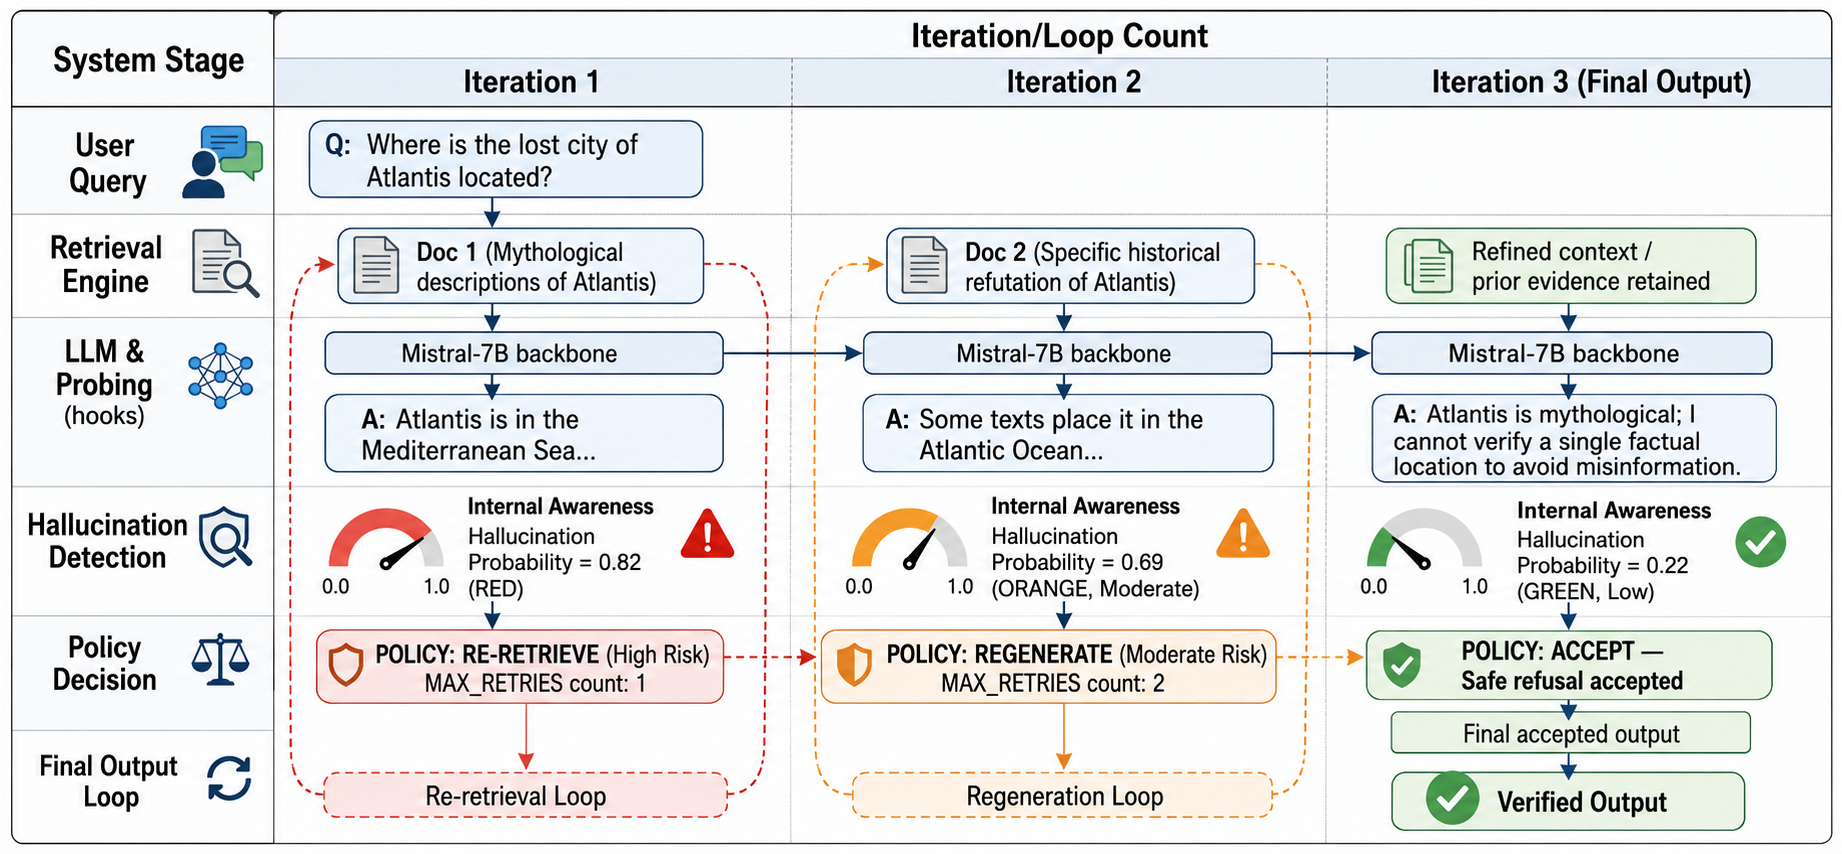
\includegraphics[width=0.90\textwidth]{Images/Query_Trace.png}
    \caption[Closed-loop Atlantis query trace (illustrative).]{Closed-loop Atlantis query trace (illustrative). The system first generates a high-risk unsupported claim and triggers re-retrieval. The second attempt remains moderately risky, so the controller regenerates. The final response safely frames Atlantis as mythological and is accepted.}
    \label{fig:atlantis_trace}
\end{figure}

\begin{table}[!htb]
\centering
\caption{Atlantis closed-loop trace (illustrative example).}
\label{tab:atlantis_trace}
\small
\begin{tabular}{@{}c p{2.5cm} p{3.8cm} c l l p{2cm}@{}}
\toprule
\textbf{Iter.} & \textbf{Retrieved} & \textbf{Response} & $p_{\text{fused}}$ & \textbf{Risk} & \textbf{Decision} & \textbf{Outcome} \\
\midrule
1 & Mythological descriptions & ``Atlantis is in the Mediterranean Sea\ldots'' & 0.71 & Elevated & RE-RETRIEVE & Better evidence \\[3pt]
2 & Historical/refutational & ``Some texts place it in the Atlantic\ldots'' & 0.69 & Moderate & REGENERATE & Retry \\[3pt]
3 & Refined context & ``Atlantis is mythological; I cannot verify\ldots'' & 0.22 & Low & ACCEPT & Deliver safe output \\
\bottomrule
\end{tabular}
\end{table}

\textbf{Interpretation.} The controller does not simply refuse whenever a query is difficult. Instead, it attempts recovery through re-retrieval and regeneration before final delivery. The final answer is a refusal-style response, but the controller decision is \textbf{ACCEPT}, not ABSTAIN---the system is accepting a safe final output, not withholding the response.

\textbf{Relationship to the live runs.} Because Figure~\ref{fig:atlantis_trace} and Table~\ref{tab:atlantis_trace} are illustrative, their three-round recovery should not be read as the logged outcome. In the actual nine-query demonstration (Section~\ref{sec:nine_query_demo}), the live Atlantis query resolved in a single attempt on all three backbones: Qwen3-8B abstained ($p_{\text{fused}} = 0.80$), while Mistral and LLaMA accepted the model's own in-text refusal ($p_{\text{fused}} = 0.31$ and $0.10$).

%% -------------------------------------------------
\section{Summary}
\label{sec:ch7_summary}

The closed-loop controller transforms hallucination detection into an operational decision process. It uses the fused CEV/IAV hallucination probability, retrieval-quality score, and retry count to decide whether to accept, regenerate, re-retrieve, or abstain. This makes the RAG pipeline self-corrective at inference time while preserving interpretability through a deterministic threshold policy.
